\documentclass[10pt,twocolumn,letterpaper]{article}

\usepackage{cvpr}
\usepackage{times}
\usepackage{epsfig}
\usepackage{graphicx}
\usepackage{amsmath}
\usepackage{amssymb}

% Include other packages here, before hyperref.

% If you comment hyperref and then uncomment it, you should delete
% egpaper.aux before re-running latex.  (Or just hit 'q' on the first latex
% run, let it finish, and you should be clear).
\usepackage[breaklinks=true,bookmarks=false]{hyperref}

\cvprfinalcopy % *** Uncomment this line for the final submission

\def\cvprPaperID{****} % *** Enter the CVPR Paper ID here
\def\httilde{\mbox{\tt\raisebox{-.5ex}{\symbol{126}}}}

% Pages are numbered in submission mode, and unnumbered in camera-ready
%\ifcvprfinal\pagestyle{empty}\fi
%\setcounter{page}{4321}
\begin{document}

\title{Applied Machine Learning Final Report}

\author{Moaz Mohamed\\
The University of Adelaide\\
Adelaide SA 5005\\
{\tt\small a1779177@student.adelaide.edu.au}
% For a paper whose authors are all at the same institution,
% omit the following lines up until the closing ``}''.
% Additional authors and addresses can be added with ``\and'',
% just like the second author.
% To save space, use either the email address or home page, not both
}

\maketitle
%\thispagestyle{empty}


%%%%%%%%% BODY TEXT
\section{Introduction}

There has been an increase of the usage of machine learning technique in medicine. From helping doctors predicting the severity of diseases \cite{Yao2020}, And using machine learning for protein folding problems \cite{Noe2020}. In this project machine learning will be used to re-purpose existing drugs to treat one of neglected tropical diseases visceral Leishmaniasis. Which is the most deadly species of the Leishmaniasis parasite.



\section{Problem Statement and Motivations}
\subsection{Leishmaniasis}

leishmaniasis is a family of diseases caused by the leishmania parasites. There are about 20 different species that are responsible for these diseases. the forefront of research and development is visceral leishmaniasis. There are also other very prevalent forms particularly cutaneous leishmaniasis and mucoucutaneous leishmaniasis. Which are more akin to skin disease issues and also post kala are dermal leishmaniasis which is a hot emerging topic in terms of the leishmania field because it seems to be a reservoir for various leishmania  parasites during the occasional droughts and peaks in the wave of the way these diseases progress. In this project we will concentrate on visceral leishmaniasis. Visceral leishmaniasis is the most severe form it's caused by a two particular parasites Leishmania donovani and Leishmania infantum. There are hundreds of millions of people at risk worldwide about 82 countries that visceral parasite is present. It's transmitted by a sand fly vector so very similar to the way malaria is transmitted by mosquitoes. Leishmaniasisis transmitted by sand flies. The symptoms for visceral leishmaniasis are severe. The symptoms are prolonged fever, an enlarged spleen and liver , anaemia and weight loss and most importantly, This is a disease that is fatal if there is no treatment. There are tens of thousands of new cases every year about half of those are found in east Africa. This is a disease that's prevalent across the globe particularly Brazil and India outside of Africa also in east Africa, south Sudan, Kenya and Ethiopia figure \ref{fig:lesh_map1}. There's also a main major problem of co-infection with HIV particularly prevalent in east Africa which exacerbates both. There's a paediatric element to this hence about 50$\%$ of the cases for this disease are in children.


\begin{figure}[h!]
  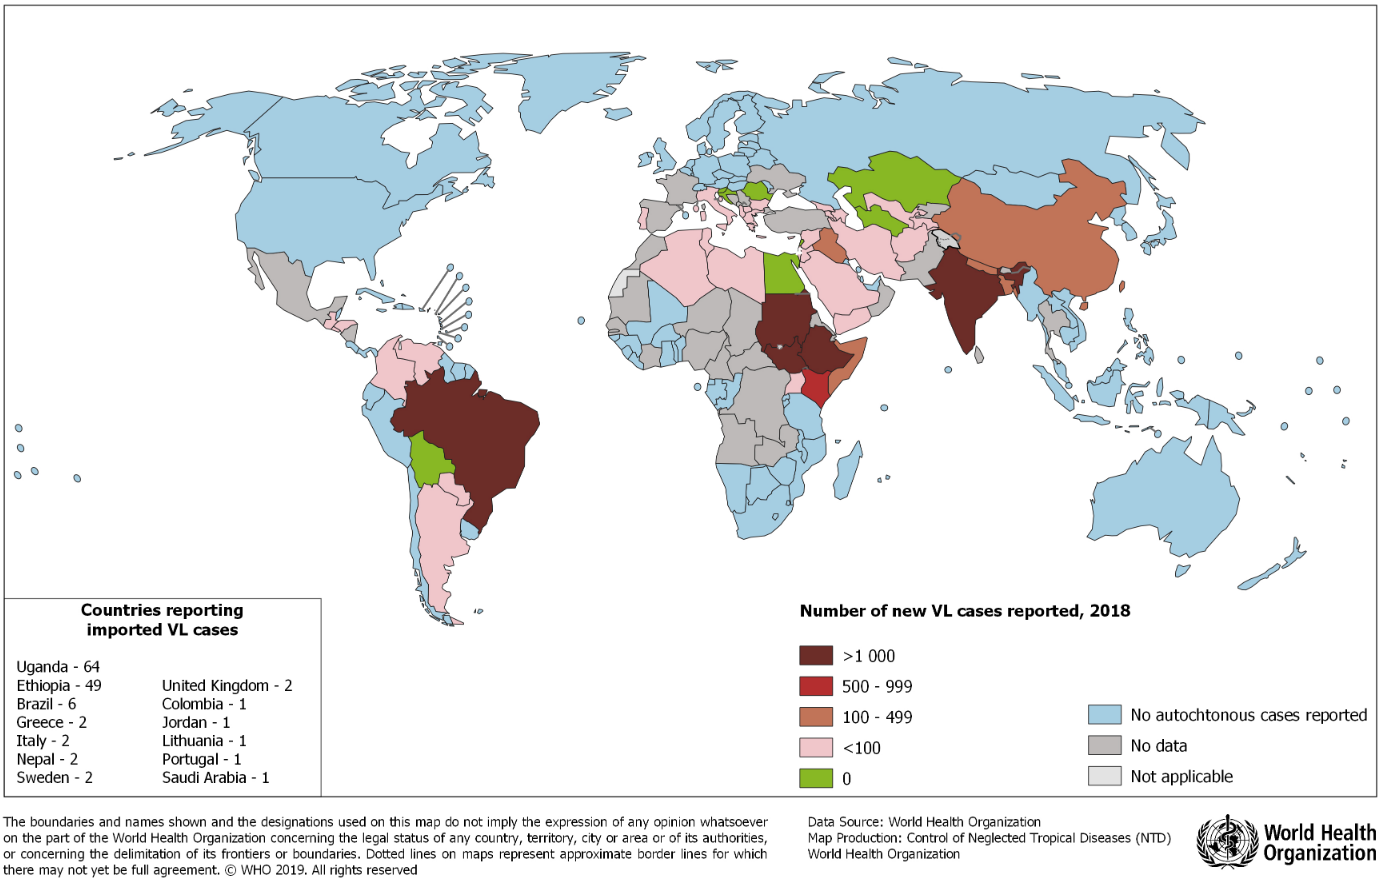
\includegraphics[width=\linewidth]{lesh_map1.png}
  \caption{Status of endemicity of visceral leishmaniasis, worldwide, 2018}
  \label{fig:lesh_map1}
\end{figure}






There are treatments available for visceral leishmaniasis figure \ref{fig:drugs_lesh}.These drugs are bad. They are hard to administer.They are not very efficacious. They are toxic. They have terrible side effects and in some cases they have issues with affordability so most of these drugs require slow IV or im infusion. They require hospitalisation for many days in some cases weeks painful administrations and side effects that are barely tolerable\cite{Arya2013}. One of these products miltefosine is orally available so it can be given as a pill but it's teratogenic so it can't be used in women of child bearing age \cite{Dorlo2012}. It also has some awful toxic toxicological side effects associated with it. There is also a big problem with the efficacy of these drugs. Depending on the region of the world whether when investigating these treatments some of them work very well particularly in Asia and in India figure \ref{fig:drugs1_lesh}. Others and particularly in Africa there is a really poor response rate even some cases as low as 50$\%$ success rate which is not good enough. There is a clear need for a new treatment. Something that is safe, efficacious, cost effective, cheap and ideally orally administered \cite{Chappuis2007}.



\begin{figure}[h!]
  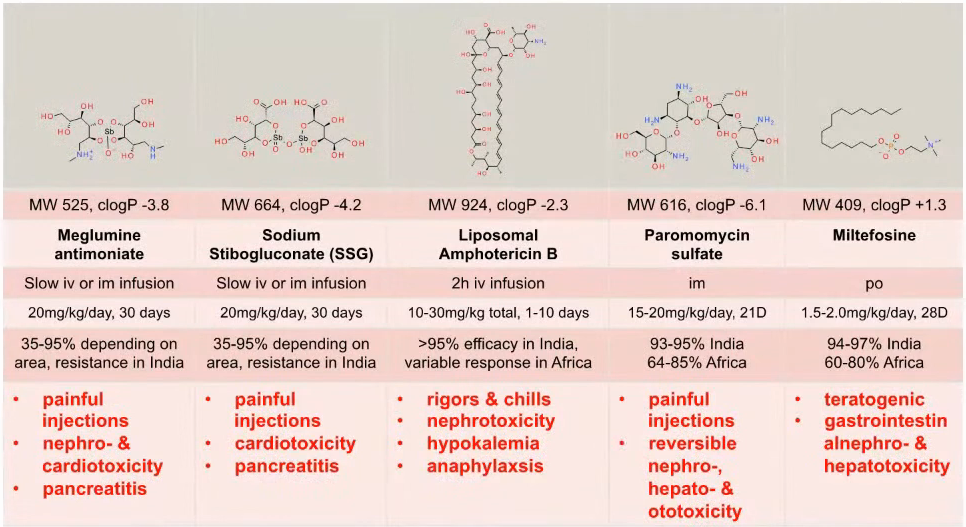
\includegraphics[width=\linewidth]{drugs_lesh.png}
  \caption{Drugs for leishmaniasis}
  \label{fig:drugs_lesh}
\end{figure}



\begin{figure}[h!]
  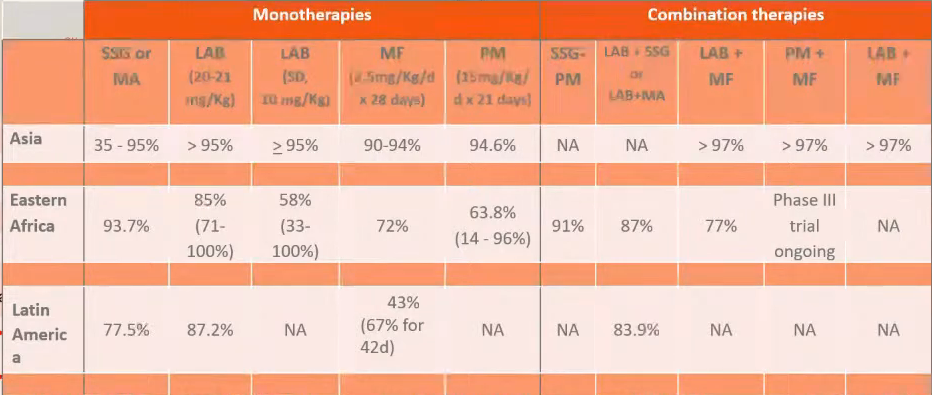
\includegraphics[width=\linewidth]{drugs1_lesh.png}
  \caption{Efficacy of drugs }
  \label{fig:drugs1_lesh}
\end{figure}




\subsection{Current and Future Drug Discovery }

 The drug development process is designed to ensure that innovative new medicines are effective, safe and available for patients in the shortest possible time. The first step in drug development is to discover the best targets for treating or preventing. A disease targets are usually proteins in the patient's body, Which are associated with a disease or proteins in microorganisms causing a disease. The challenge is to identify which proteins are relevant and more importantly confirm their role in a disease. Increasingly Researchers focuses on understanding cellular networks of proteins or pathways a single protein may transmit messages to several other proteins sometimes in multiple pathways affecting their function knowing how these pathways work and interact helps to identify the most appropriate target for a drug. The pathway approach allows researchers to better understand the mechanisms of a disease. This knowledge determines the priorities in target discovery. In drug discovery several methods like high-throughput screening and computer-based design are used to find chemical compounds or biologics that bind to the identified target figure \ref{fig:drugs_recep}. If a compound modulates the target in a way that is expected to alter the disease this so-called hit will be refined to improve its safety and effectiveness eventually becoming a drug candidate.



\begin{figure}[h!]
  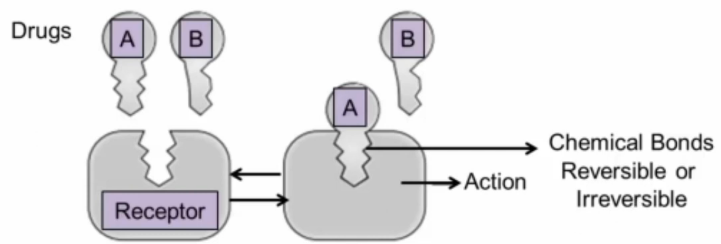
\includegraphics[width=\linewidth]{drugs_recep.png}
  \caption{Drug and target protein }
  \label{fig:drugs_recep}
\end{figure}




 Discovering and bringing one new drug to the market typically takes an average of fourteen years of research \cite{Zurdo2013} and clinical development efforts and costs around two billion u.s. dollars of 10,000 or more in figure \ref{fig:drug_valley}. Hits tested in early drug discovery only one may eventually lead to a drug that reaches the market in the late preclinical stage. Further experiments are conducted on the drug candidate to ensure it is safe for patients and has the required pharmacokinetic properties like appropriate absorption and metabolism by the human body. These experiments are executed with extraordinary diligence to minimise any risks to human test subjects. the goal of this project is to investigate the ability of machine learning methods to speed up the process of drug discovery with addition to finding a drug is that is already available in the market to reduce the time from research to deployment. Hence repurposing existing drugs can shave some time at the clinical trial phase. 

\begin{figure}[h!]
  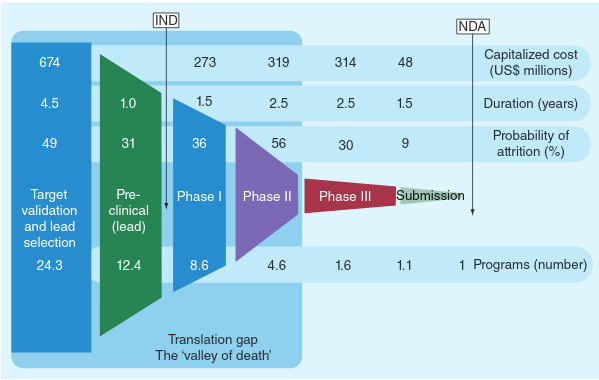
\includegraphics[width=\linewidth]{drug_valley.png}
  \caption{Drug Discovery timeline }
  \label{fig:drug_valley}
\end{figure}


\section{Machine learning novelty in drug discovery}
\subsection{The case for Graph Networks}

Concerning drug design and what enables machine learning to do anything interesting in terms of automation is the richness in the data. In simple property prediction tasks if we have a molecule and  we want to understand its properties in terms of solubility toxicity and others. In order for machine learning method to try to uncover the underlying physical relationship between the molecule and the associated properties. We need to have the data rich enough so that it exercises this mapping.There's tons of data already available and being generated through small and large scale assays and curated database. 

The task framed ambitiously is to take a precursor molecule and translate it into another precursor that satisfies design criteria and learn to do that from examples. There are a few key challenges. In order to achieve that we have to somehow either explicitly or implicitly be able to predict properties of molecules figure \ref{fig:learn.png}, Otherwise how could we search for a better molecule, So we solve it as a machine translation problem in one step going from the starting molecule to the molecule that has better properties. For predicting molecular properties many of the current approaches are now machine learning based. The key problem is to try to somehow look at the model molecule learn to read the molecule in the way that highlights the intricate features or combinations of features in the molecules, That drive the properties that it has, and we need to learn to read molecules properly to try to explicate properties of molecules learn to explicate those properties at multiple different levels of resolution. 


\begin{figure}[h!]
  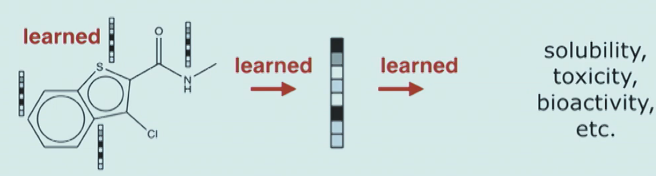
\includegraphics[width=\linewidth]{learn.png}
  \caption{Graph and Vector representation }
  \label{fig:learn.png}
\end{figure}



A molecular graph is a 2d graph in figure \ref{fig:graph_learn1}. What we would like obtain is a representation of a vector. Representation for each atom that somehow captures the context in which it appears in this molecule. In order to achieve that we somehow have to communicate the context around that atom to the atom itself. What we are going to do is to lay out a set of possible ways to solve this problem and drive the selection of which way is best based on their end task that We are trying to solve, So a way of aggregating the features from the context it's useful if it helps to solve the end task in our case predicting molecular properties, So we're going to communicate send messages between the atoms here to get a vector representation for each atom \cite{Gilmer2017}.


\begin{figure}[h!]
  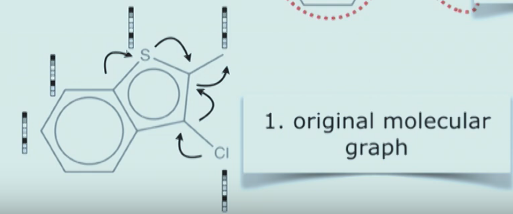
\includegraphics[width=\linewidth]{graph_learn1.png}
  \caption{Sub Structure 1 }
  \label{fig:graph_learn1}
\end{figure}



in figure \ref{fig:graph_learn2}. We step up one level further look at larger sub structures that appear in molecule and how they are linked together and obtain a vector representation not for each atom but for each sub structure in in that structure. Similar to what we have done before. We are going to drive that representation based on what's around it and what other sub structures are related to it as well as what atoms those sub structures underlie. 

\begin{figure}[h!]
  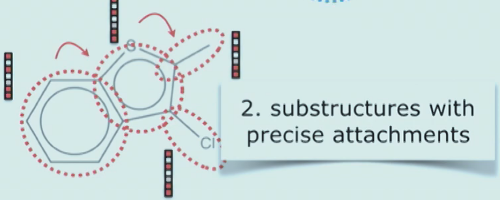
\includegraphics[width=\linewidth]{graph_learn2.png}
  \caption{Sub Structure 1 }
  \label{fig:graph_learn2}
\end{figure}


Finally we have highest level of representation which is sort of a loosely connected sub structures, Although losing information about the intricate connections between these larger pieces but retaining some information about what they are and how they are roughly connected. We could add a stack of vector representations at multiple different levels of resolution and that is the representation for the molecule, The way these are learned then get examples of molecule properties. The predictions are mediated by these multi resolution representations\cite{Hamilton2017}.

%-------------------------------------------------------------------------
\subsection{Chemical compounds representation}
The usage of machine learning in ligand based screening require having the lest amount reduction in information when representing a chemical compound. A popular representation method called Simplified molecular-input line-entry system (SMILES), Its a one line notation encoding of a molecular structure. Another representation is graphs. Edges can have weights associated with how strong the bond is and each node can have a feature vector that can encode specific attributes for each node as each node represent a chemical element. Whereas in SMILES only the elements and the bonds are encoded hence graphs is a better tool for representing chemical compounds \cite{Toropov2011}. 
%------------------------------------------------------------------------


\subsection{Graph Neural Network}

There are challenges on performing convolution operation on graphs due to the complex nature of graphs and the fact that with the different representation of graphs we can have different adjacency matrix hence the requirement of locality and aggregation of convolution isn't met \cite{Kipf2017}. 


\begin{figure}[h!]
  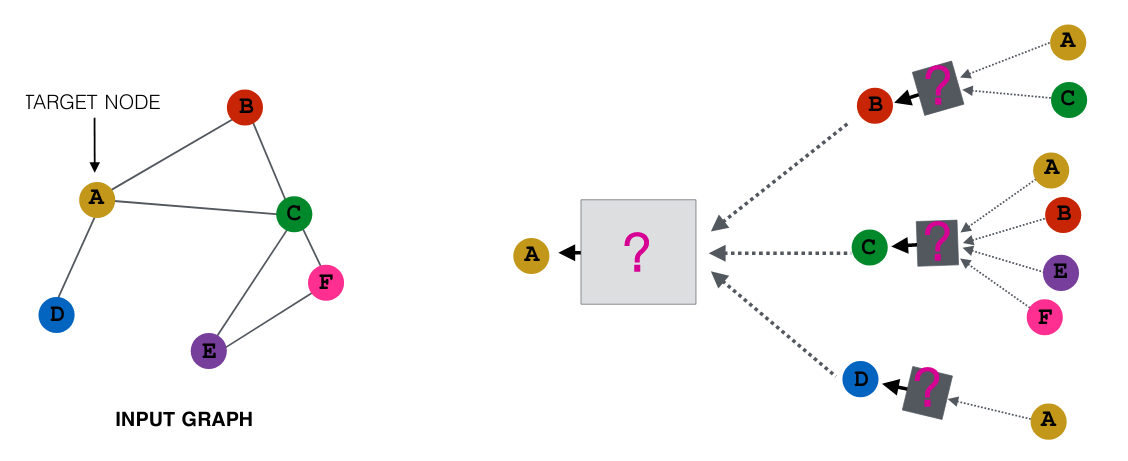
\includegraphics[width=\linewidth]{graph.png}
  \caption{Graph Computational Model}
  \label{fig:graph}
\end{figure}


Different strategy is needed to apply different deep learning frameworks on graphs. In 2017 on " Neural Message Passing for Quantum Chemistry" \cite{Gilmer2017} outlines and summarized different machine learning methods to apply convolution or commonly what is known in graphs machine learning community as massage passing. The key idea is to use encoder like structure as having lower the dimensionality of a node. That is done by aggregating massages from the target node neighbours then applying a learn-able weight matrix and bias to encode the graph features into a lower dimension. By summing the feature vectors that are connected to the targeted node and multiplying it with a learn-able and differentiable weight matrix. Its important to note that the summation operation is order invariant and the notion of depth instead of adding more layers as in typical neural network instead of Graph neural network we are borrowing information from more nodes or going deeper in the graph network to compute the summation and finally after applying the weight matrix and the activation function. We are left with a node embedding 


\begin{equation}
\mathbf{h}_{v}^{k}=\sigma\left(\mathbf{W}_{k} \sum_{u \in N(v)} \frac{\mathbf{h}_{u}^{k-1}}{|N(v)|}+\mathbf{B}_{k} \mathbf{h}_{v}^{k-1}\right)
\end{equation}

 

\subsection{Aggregation variants}

In GraphSage paper \cite{Hamilton2017}. Instead of adding both the weight and the bias. The authors concatenated both terms and let the Back-propagation decide which term is more important ${W}_{k}$ or ${B}_{k}$, also the aggregation method isn't limited to finding the mean of the neighbors feature vectors. A pooling or applying a LSTM can be utilized and in the GraphSage paper using different aggregation resulted in better performance.  


\begin{equation}
\mathbf{h}_{v}^{k}=\sigma\left(\left[\mathbf{W}_{k} \cdot \operatorname{AGG}\left(\left\{\mathbf{h}_{u}^{k-1}, \forall u \in N(v)\right\}\right), \mathbf{B}_{k} \mathbf{h}_{v}^{k-1}\right]\right)
\end{equation}

\begin{equation}
\mathrm{AGG}=\gamma\left(\left\{\mathbf{Q h}_{u}^{k-1}, \forall u \in N(v)\right\}\right)
\end{equation}

\begin{equation}
\mathrm{AGG}=\mathrm{LSTM}\left(\left[\mathbf{h}_{u}^{k-1}, \forall u \in \pi(N(v))\right]\right)
\end{equation}



\subsection{Edge Memory Graph Neural Network}

\begin{figure}[h!]
  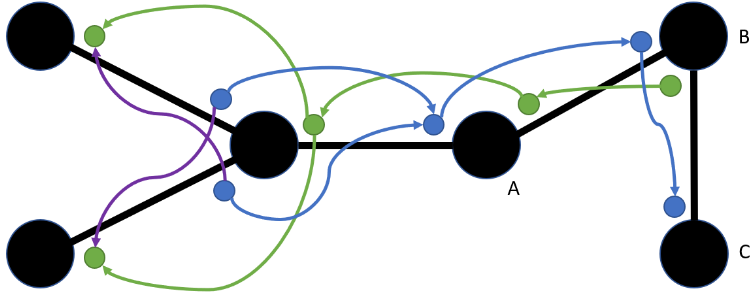
\includegraphics[width=\linewidth]{edge.png}
  \caption{Edge Memory Graph Neural Network}
  \label{fig:graph}
\end{figure}

In the message passing frame work. The data is aggregated from neighbouring atoms to compute the message to a centre atom. Instead of having a hidden state in the node. The hidden state will be in each directed edge. In a node to node connection the directed graph will have two directed edges which coincide to two hidden states. The update scheme of the hidden state of the edges will be updated according to which heads close to its tail \cite{withnall2019}. 

In each edge the follow of information is directional as massages flow from a tail node to a head node. Hidden states of edges are taken into consideration when updating an edge $(v, w)$ of the directed graph $G=(V, E)$ is

$$
S_{v w}^{(t)}=\left\{h_{k v} \mid k \in N(v), k \neq w\right\}
$$

Before massage passing happens, An embedding of an edge feature is created by combining the edge and the node feature vectors of the two node features through a FFNN 
$$
e_{v w}^{\prime}=f_{N N}^{e m b}\left(\left(e_{v w}, h_{v}^{(0)}, h_{w}^{(0)}\right)\right)
$$

At (t=0), $e_{v w}$ is the raw bond feature and $h_{v}^{(0)}$ is the atom feature vector. $h_{v w}^{(t)}$ is the edge hidden state of $(v, w)$ at time t and its updated by equations 

\begin{equation}
\left\{\begin{aligned}
m_{v w}^{(t)} &=A_{t}\left(e_{v w}^{\prime}, S_{v w}^{(t)}\right) \\
h_{v w}^{(t+1)} &=U_{t}\left(h_{v w}^{(t)}, m_{v w}^{(t)}\right)
\end{aligned}\right.
\end{equation}

Its important to note that a static edge feature $e_{v w}^{\prime}$ and time modulated edge state $h_{v w}^{(t)}$ is contributing and in a directed edge. A vector of zeros is instantiated in $h_{v w}^{(0)}$. An attention $A_{t}^{e}$ function is the choice of an aggregation. All the edges involving node $v$ including the edge $(v, w)$ itself is $S_{v w}^{\prime(t)}$. 


\begin{equation}
A_{t}^{e}\left(e_{v w}^{\prime}, S_{v w}^{(t)}\right)=\sum_{x \in S_{v w}^{(t)}} f_{N N}(x) \odot \frac{\exp \left(g_{N N}(x)\right)}{\sum_{x^{\prime} \in S_{\nu W}^{(t)}} \exp \left(g_{N N}\left(x^{\prime}\right)\right)}
\end{equation}

where 

$$
S_{v w}^{\prime(t)}=S_{v w}^{(t)} \cup\left\{e_{v w}^{\prime}\right\}
$$



\begin{equation}
h_{v w}^{(t+1)}=\operatorname{GRU}\left(h_{v w}^{(t)}, m_{v w}^{(t)}\right)
\end{equation}




\section{Preparing data and loss function}


In this project we will be targeting visceral Leishmaniasis for the strain of Leishmania donovani (strain BPK282A1). Going through the research literature in Leishmaniasis Research (Methionyl-tRNA synthetase protein) has been identified as a viable target \cite{Barrett2012} \cite{T.Jacobs2011}. Successfully binding or inhibiting Methionyl-tRNA synthetase will starve Leishmaniasis parasite from an important biological function for its survival. Another criteria that supports targeting this protein is the amount of assay data available for this protein target. Close 70,000 assays with their inhibition values are available for research purpose in European Bioinformatics Institute, of the European Molecular Biology Laboratory (ChEMBL). In addition to 9,800 drugs that are in trial have been curated from PubChem, DrugBank database and The National Center for Biotechnology Information (NCBI). The binding affinity or inhibition value will be predicted for Methionyl-tRNA synthetase protein.


RDKit will be used to turn the smiles notation into graph representation and to generate the feature vectors for the edge. DeepChem will be used to provide atom feature vector. Since binding affinity is what is required for this project as a continuous prediction as a regression task the mean squared error will be used as a loss function.


\section{Results and Limitations }

\subsection{limitation}

the Usage EMNN was halted due to low computational resources. Due to the large data-size one epoch took one hour. EMNN needs around 300-450 epochs. An alternate approach was devised to realise some if not all project goals. Instead of using GNN to represent compounds RdKit was used to extract as much features as possible for every chemical compounds such, "HeavyAtomCount", "RingCount", "NumValenceElectrons" and "NumRotatableBonds". A total of 14 features have been extracted and tabulated in tabular format. Gradient Boosting methods are known for their good performance on tubular data but instead of using XGBoost and alike methods Attentive Interpretable Tabular Learning (TabNet) was used instead. That selection was due to its ability to match if not outperform gradient boosting methods in regression tasks \cite{Arik2019}. 

\subsection{TabNet}

 The architecture in figure \ref{fig:tab1} starts with a bottom layer for the raw input features through a bottom layer. There are number of steps (hyper parameter) and all the steps are the same. For each step there are feature transformer blocks and attention attentive transformer blocks that creates a mask  for the features for the next feature transform block (2) and then each feature transform of that creates boost predictions. The next feature is for the the attentive transformer(2) so the output of the model are summed such that every step sums their predictions. Finally, A final layer (FC) allows to make any of a type of problems/predictions. 

\begin{figure}[h!]
  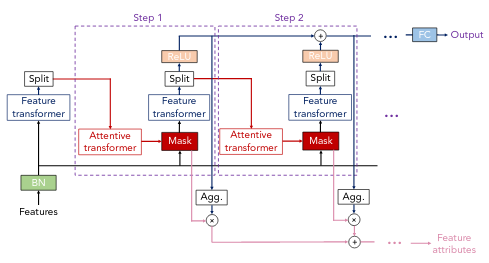
\includegraphics[width=\linewidth]{tab1.png}
  \caption{TabNet encoder architecture}
  \label{fig:tab1}
\end{figure}

The feature transformer block in figure \ref{fig:tab2}. This is an example of four consecutive gate linear unit (GLU) blocks. One feature transformer is just a fully connected layer followed by a bottom layer and then a gated linear unit activation. The gated linear unit activation is a sigmoid times a the input features and this is a bit wise multiplication. 
$$
G L U(x)=\sigma(x) \odot x
$$
Its important to note that, There are some shared blocks and independent blocks. The idea is that in every step the two first GLU blocks are going to be shared across all steps others are dependent so model is sharing some weights across different steps. There is a skip connection at every GLU block as the initial input through next step and this allows TabNet to train deeper models and allows for a smooth training.  

\begin{figure}[h!]
  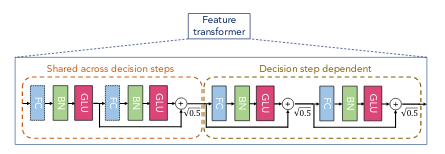
\includegraphics[width=\linewidth]{tab2.png}
  \caption{Feature transformer}
  \label{fig:tab2}
\end{figure}



Attentive transformer in figure \ref{fig:tab3}. It's a fully connected layer then Batch-Norm and a prior scale and sparse Max. The idea of prior is that at the beginning of the training the prior is going be all ones and the prior is giving indications about the features and how much have we have used them in the previous step. At the beginning they are no knowledge about the features so the prior is all one then for the next steps the prior is going to be a multiplication of all the previous steps.

$$
P_{0}=1
$$

it's gamma minus the previous masks 
$$
P_{i}=\prod_{j=1}^{\prime}\left(\gamma-M_{j}\right)
$$

If gamma is set  close to one this allows the model not to use the same features at every different steps. Hence,  Setting a gamma close to one the model have different features for every steps. If gamma is set a large number the model will reuse the same features at every step. 





\begin{figure}[h!]
  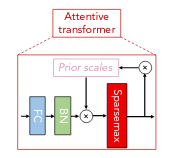
\includegraphics[width=\linewidth]{tab3.png}
  \caption{Attentive transformer}
  \label{fig:tab3}
\end{figure}

\section{Results}
Hyper-parameter optimization have been preformed using the Grid Search method for the Tabnet model to select the best parameter for this project. Adam optimizers have been utilized with a learning rate of 2e-2 and a exponential learning scheduler. A max epoch number of 1000 was selected while using early stopping with a patience value of 50 to save time. Only the best model is saved. After the optimization the lowest mean squared error on the validation set was (0.4721) and (0.4648) on the testing set. This not ideal as they are numerous works that could achieved better in terms of lower error values using GNN. Although Never on a dataset of this size. 



\begin{figure}[h!]
  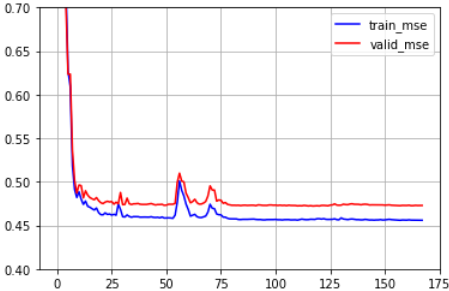
\includegraphics[width=\linewidth]{results.png}
  \caption{Train-Test MSE curve}
  \label{fig:graph}
\end{figure}


\begin{table}[htb]
\centering
\begin{tabular}{|l|l|l|l|} 
\hline
Hyper-parameter     & Best Value & range  \\ 
\hline
n-dimensions   & 32 & [16,32,64]    \\ 
\hline
n-attention   & 32 &  [16,32,64]   \\ 
\hline
n-independent blocks  & 4   & [2,3,4]  \\
\hline
n-shared blocks    & 4  & [2,3,4]  \\
\hline
n-steps     & 4  &   [2,3,4] \\
\hline
Learning rate     & 2e-2  &  [2e-2,2e-3,2e-4]  \\
\hline
\end{tabular}
\caption{Hyper-parameter selection}
\label{tab:class_per}
\end{table}

the Best trained model has been used to make prediction on the drugs on trial dataset and top 20 preforming candidates have been extracted and visualized. To validate the results of the model AutoDock Vina has been used to simulate the performance of the compounds on the targeted protein. Unfortunately most of the top preforming candidates couldn't be simulated due to AutoDock inability to dock chemical compounds with torsion angles more than 32. Flexible docking could be preformed but at the risk of destroying secondary structure. Proper flexible docking require the knowledge of Chemical kinetics which outside of the scope of this project. Regardless, the model predicted (4-(Benzylideneamino)benzenesulfonamide) as a molecule with relatively good inhibition score. Fortunately, The compound has only 16 torsion angles so a rigid docking could be preformed. The predicted molecule successfully docked with a blind docking figure. The docking simulation resulted in docking score of -4.71. Which is a promising score that prompts more investigation and trying different docking procedure such as flexible docking. The output Report of this simulation will be provided in the appendix. 



\begin{figure}[h!]
  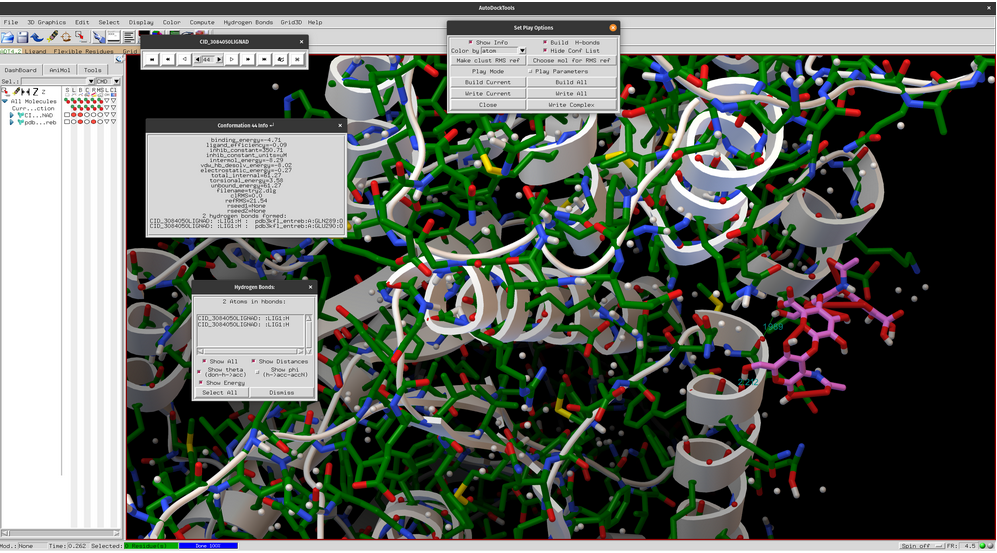
\includegraphics[width=\linewidth]{vina1.png}
  \caption{Auto Dock Report of the docking}
  \label{fig:graph}
\end{figure}



\begin{figure}[h!]
  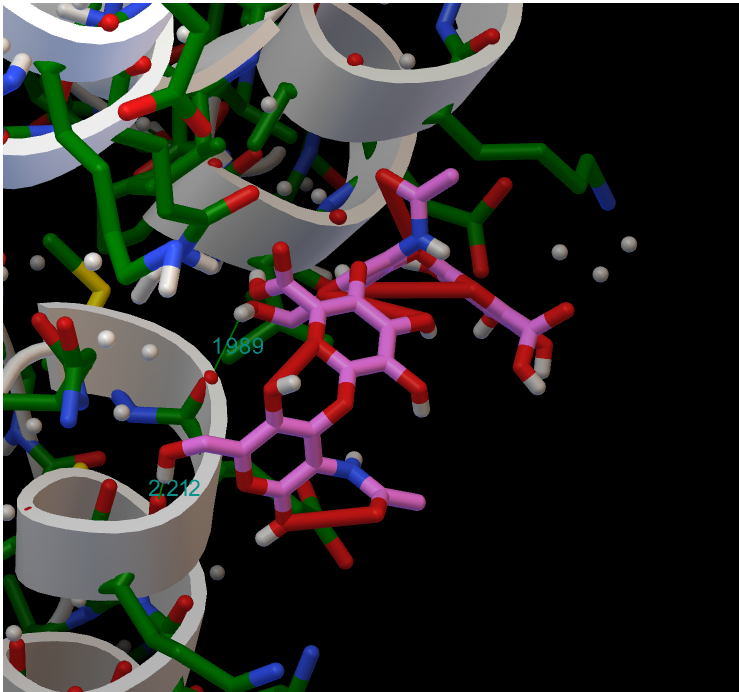
\includegraphics[width=\linewidth]{vina2.png}
  \caption{ligand docking at binding site}
  \label{fig:graph}
\end{figure}

\section{Conclusion}
Deep learning has disturbed many technological sectors and the pharmaceutical sector is no different. A typical drug discovery projects takes years to come up with a few viable compounds that could be optimised and tested in trial. Due to deep learning and particularly GNN that time span could be reduced in months. Although a promising compound that would be taken into the optimisation stage should have a scoring value of -8.0 or less. A molecule with a score of -4.71 that did bind to the protein target was found with a non optimal machine learning method. Hence the representation power of GNN are suited to be used for drug discovery purposes and hence would have generated better predictions. 

\section{Future Work}
Ideally GNN are most suited to represent chemical compounds but due too limited computation resources that plan had to halted. That problem could be mitigated using cloud service providers such AWS or azure as more resources could be allocated dynamically. In addition to that majority of the predicted compounds couldn't be simulated properly. AutoDock Vina was used due to its simplicity and its flexibility working with variety of file formats but due to its limitation at rigid docking and its not suitable for docking large molecules. Alternatively, A dedicated protein docking program/server should be used instead of autodock. ZDock an automatic protein docking server or HexDock a CUDA enabled protein docking program.  


\section{Notes}
Special thanks goes to Rudrarup Bhattacharjee,  PhD student, Adelaide Medical School working on Investigating the Role of TREX mRNA Export complex in Neurodevelopmental Disorders and  Dr, Rayzel Fernandes, PhD at Adelaide University and Research Associate, Imperial College London working on Targeting androgen receptor signalling in prostate cancer. For their guidance and advice. 
It has been a pleasure working in a field that is completely different to my main field (Electrical Power Engineering). As this projects enabled me to explore new areas in the machine learning research field.

{\small
\bibliographystyle{ieee_fullname}
\bibliography{egbib}
}

\end{document}
